\chapter{Simulating Chemical Kinetics Without Differential Equations}
\label{chapter4}
Most of the contents of this chapter are reprinted, with permission, from \
\begin{enumerate}
\item[\cite{ch4_10_bai2016sum}] Bai, S., \& Skodje, R. T. The Sum Over Histories Representation for Chemical Kinetics: A Quantitative Theory Based on Chemical Pathways. \textit{International Reviews in Physical Chemistry}, 35(4), 539-567. \textbf{2016}
\item[\cite{bai2017simulating}] Bai, S., \& Skodje, R. T. Simulating Chemical Kinetics Without Differential Equations: A Quantitative Theory Based on Chemical Pathways. \textit{The Journal of Physical Chemistry Letters}, 8(16), 3826-3833. \textbf{2017}
\end{enumerate}

\section{Abstract}
\label{ch4:sec:abstract}
A new approach is presented for simulating the time-evolution of chemically reactive systems.  This method provides an alternative to conventional modeling of mass-action kinetics that involves solving differential equations for the species concentrations.  The method presented here avoids the need to solve the rate equations by switching to a representation based on chemical pathways.  In the Sum Over Histories Representation (or SOHR) method, any time-dependent kinetic observable, such as concentration, is written as a linear combination of probabilities for chemical pathways leading to a desired outcome.  In this work, an iterative method is introduced that allows the time-dependent pathway probabilities to be generated from a knowledge of the elementary rate coefficients thus avoiding the pitfalls involved in solving the differential equations of kinetics.  The method is successfully applied to the model Lotka-Volterra system and to a realistic H$_2-$O$_2$ combustion model.

\section{Introduction}
\label{ch4:sec:intro}
Simulation of chemical reaction networks using mass-action chemical kinetics provides an invaluable tool for uncovering chemical mechanisms and predicting time-dependent chemical behavior as functions of controllable parameters such as temperature, pressure, and initial concentrations.  As chemical mechanisms grow large, such as for hydrocarbon combustion, the resulting kinetic behavior can become quite difficult to physically decipher and, in some cases, the simulations themselves can bog down due to the proliferation of species and the need for small time steps owing to the existence of multiple time scales.  Thus, considerable effort has been devoted in the disciplines of chemistry, biochemistry, physics and engineering to interpreting and simplifying kinetic behavior in complex networks.
\newline
\paragraph{}
The usual computational approach to mass-action kinetics involves constructing and solving a set of differential equations in the continuous concentration variables $X_i(t)$ that model the local rates of formation and destruction of each of the N chemical species, $S_i$. (Underpinning kinetics equations are defined in eqns. \ref{ch2:eqn2} and \ref{ch2:eqn3}.) For the M elementary reaction steps, defined in eqn. \ref{ch2:eqn1}, the explicit rate laws $R_j(\mathbf{X})$ are provided by an external experimental or theoretical determination and $v_{i,j}$ are known constants.\cite{ch4_1_laidler1987chemical,ch4_2_steinfeld1989chemical,ch4_3_pilling1996reaction} This representation is properly regarded as a mean field theory that becomes valid in the thermodynamic limit.   For systems involving very low concentrations or strong local environment effects, more intensive simulations may be used that employ stochastic or Monte Carlo algorithms that may account for the influence of fluctuations.\cite{ch4_4_mcquarrie1967stochastic,ch4_5_gillespie1976general,ch4_6_kampen2007langevin}
\newline
\paragraph{}
In this paper, we propose a new method to simulate the kinetics of general nonlinear mechanisms that builds on, and fundamentally extends, our earlier work.\cite{ch4_7_kramer2014following,ch4_8_bai2014sum,ch4_9_bai2015sum,ch4_10_bai2016sum} In contrast to the local rate equation approach to kinetics, we propose a self-contained global method based on chemical pathways that tracks molecules and fragments as they move throughout the network.  A pathway follows a chemical moiety, at a molecular level, as it hops from species to species under the influence of elementary chemical steps. A convenient approach to the unique specification of a chemical pathway utilizes an atom-following algorithm.  If, e.g., the carbon-atom in a CH$_4$ reagent is initially “tagged”,  $\textcolor{red}{\textbf{C}}\text{H}_4(+\text{OH}) \xrightarrow[\text{R}_{1}]{\makebox[0.6cm]{}} \textcolor{red}{\textbf{C}}\text{H}_3 (+\text{OH})  \xrightarrow[\text{R}_{2}]{\makebox[0.6cm]{}} \textcolor{red}{\textbf{C}}\text{H}_2 (+\text{O}) \xrightarrow[\text{R}_{3}]{\makebox[0.6cm]{}} \textcolor{red}{\textbf{C}}\text{H}_2\text{O}$ defines a three-step pathway leading from CH$_4$ to the product CH$_2$O.  Each reaction is modeled as a random event governed by transition probabilities obtained from the elementary rate laws.  By constructing paths for a complete set of atoms in the initial state at a time $t_0$, it is possible to predict the subsequent values of any kinetic observable given the pathway probabilities (see below).  Hence, the method is global in the sense that it replaces local rate equations based on instantaneous rates for individual species with expressions that span the entire network over finite times using multistep chemical pathways.
\newline
\paragraph{}
The use of chemical paths to analyze the behavior of chemical networks has a long history.  A most convenient way to visualize and enumerate chemical paths involves the use of graph theory.\cite{ch4_11_mekenyan1994graph,ch4_12_balaban1976chemical,ch4_13_garcia2008some} Graph theoretic analysis of chemical mechanisms was initiated by the early work of Christiansen\cite{ch4_14_christiansen1953elucidation} and also King and Altman\cite{ch4_15_king1956schematic} who exploited the analogy between chemical and electrical circuit theory.  Since then, there have been numerous treatments of chemical networks, especially for biochemical systems, that have demonstrated the utility of graph theory.\cite{ch4_16_oster1971network,ch4_17_hill1966studies,ch4_18_fishtik2004reaction,ch4_19_he2008graph,
ch4_20_lehmann2004algorithm,ch4_21_feng2010dominant,ch4_22_lu2006applicability} Closely related work on the solution of master equations via network analysis has also been explored using graph theory.\cite{ch4_23_schnakenberg1976network,ch4_24_andrieux2007fluctuation} Much of work on kinetic graphs has focused on the developing expressions for the steady state rates for first-order or pseudo-first-order chemical mechanisms.  Typically, the vertices of those graphs comprise a subset of the species, such as biochemical intermediates, and the edges are reaction steps.  Quantitative treatment of the kinetics are possible using edge weights obtained from the steady state fluxes.
\begin{figure}[htbp]
	\caption[A schematic representation of a time-dependent pathway]{A schematic representation of a time-dependent pathway
followed by a tagged atom through a chemical network of five species.
The reactions occur instantaneously at times $t_1$, $t_2$, $t_3$, and $t_4$, which are
randomly selected and averaged to obtain the pathway probability.}
    \begin{center}
	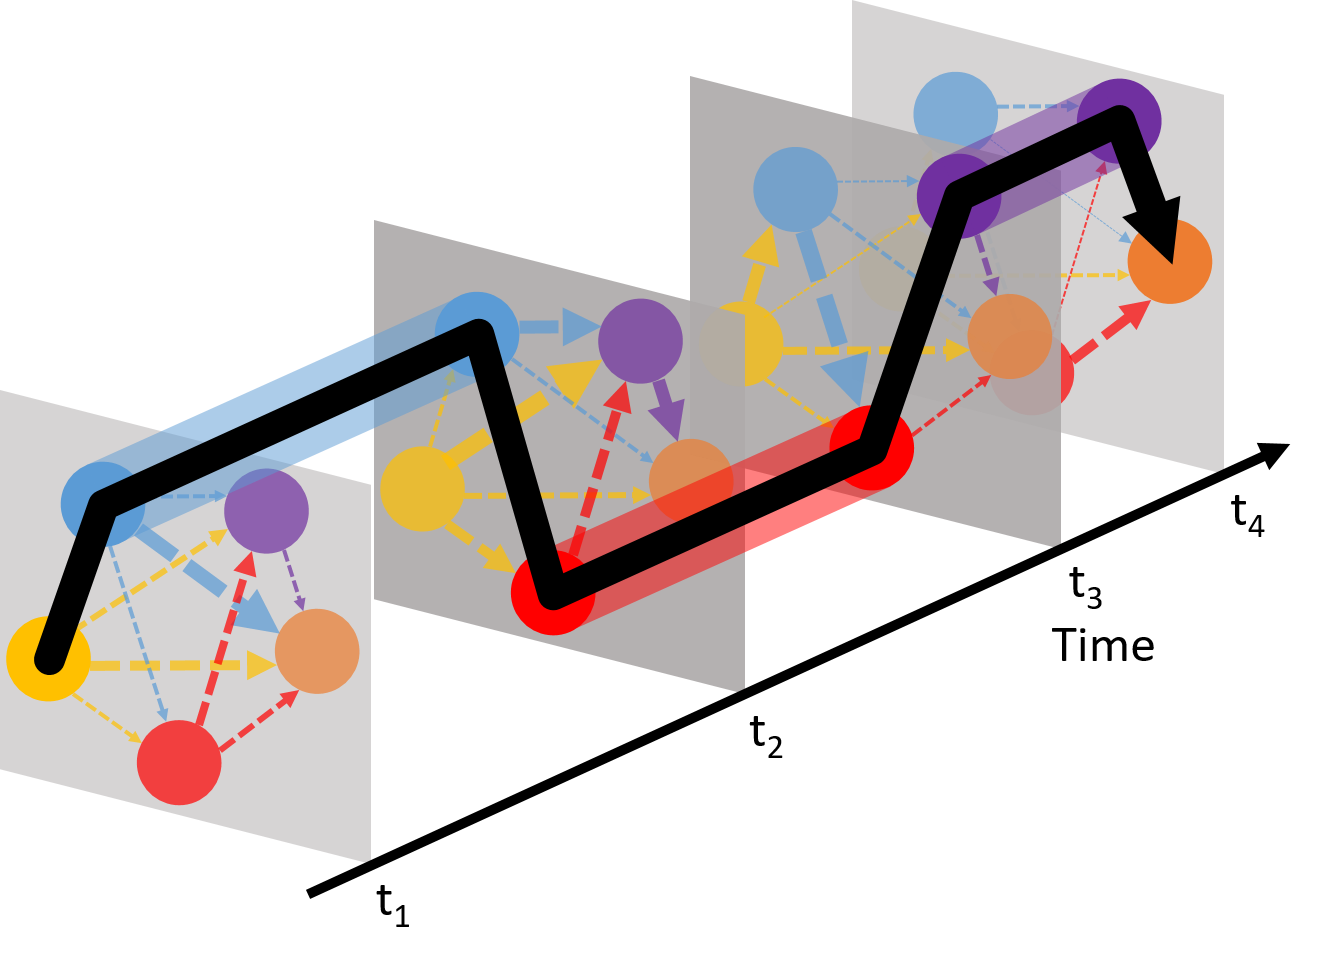
\includegraphics[width=100mm]{figs/chapter4/fig1.png}
    \end{center}
\label{ch4:fig:1}
\end{figure}
In our work, we have developed a quantitative pathway
analysis, called the Sum Over Histories Representation or
SOHR, which goes beyond steady state conditions and fully
embraces the time-dependent and nonlinear behavior of
general mechanisms. As emphasized in the schematic diagram
of Fig. \ref{ch4:fig:1}, the SOHR method employs time-resolved chemical pathways in which reaction occur at specific randomly selected
times. This treatment employs dynamical graph theory\cite{ch4_25_harary1997dynamic} in
which the edge weights are time-dependent. This is quite
important for quantitative modeling since static snapshots of
the reactive flow can be very deceptive for interpreting and
modeling time-dependent chemical flux. Our approach draws
inspiration from Feynman’s path integral representation of
quantum mechanics.\cite{ch4_26_feynman2010quantum} We have previously used the SOHR
method to interpret the workings of several kinetic networks,
including those involved with surface catalysis and combustion.
While we could readily identify and quantify the important
chemical paths that guided the kinetics, the results were
interpretative rather than predictive. That is, for general
nonlinear problems, the determination of the pathway
probabilities requires a knowledge of the time-dependence of
the pseudo-first order rate coefficients which, in turn, requires
an a priori knowledge of the concentrations versus time. For
interpretive analysis, the nonlinear kinetics was first solved
using conventional kinetics to obtain a reference trajectory,
$\mathbf{X}(t)$, and then the kinetics was decomposed into contributing
pathways. In this work, we overcome this limitation and formulate the SOHR as a predictive theory that does not
require a solution to eqn. \ref{ch2:eqn2}. In this way, the need to solve the
usual differential equations of mass action kinetics is avoided,
and the pathway probabilities can be solved in a self-consistent
manner.
\newline
\paragraph{}
The key to our formulation is the use of an iterative solution
technique to obtain the pathway probabilities. Here The iterative SOHR
method is presented. Given a set of chemical pathways, the
pathway probabilities and the species concentrations are
obtained simultaneously by the iteration. A strategy to identify
the most important chemical pathways is given. The new
predictive SOHR method is numerically tested on the Lotka$−$
Volterra model and H$_2-$O$_2$ combustion system. The results
presented demonstrate that the method is accurate and quickly
convergent. We conclude with a discussion of the possible
advantages of the new method.
\section{The Predictive SOHR Method}
For a linear kinetic network, the SOHR formulation is automatically predictive
since the pathway probabilities are known analytically via eqn. \ref{ch2dot5:eqn1}.
Thus, if a sufficient number of pathways are enumerated, the
sums in eqn. \ref{ch2:eqn16} are guaranteed to converge to the correct
concentration functions. However, we can immediately see a
difficulty in applying this formalism to general nonlinear kinetic
networks. Namely, the quantities Ai,m(t) are no longer constants
and pathway probabilities seen to require the solution to the
conventional kinetics eqn. \ref{ch2:eqn2} as input into eqn. \ref{ch2:eqn11}. In a departure
from our previous work, we now show how this requirement
can be avoided using a new methodology.
\newline
\paragraph{}
We shall assume that a finite number of distinct pathways, $J$,
is adequate to accurately describe the evolution of the N species
concentrations $X_i(t)$ over a time interval $t \in (0, T)$ . In the next
paragraph, we discuss how those pathways may be identified. If
the concentrations $X(t) = \left(X_1(t),\cdots,X_N(t)\right)$, which solve eqn. \ref{ch2:eqn2}
with initial conditions $\mathbf{X}(t = t_0) = {\textbf{X}}_0$ are known, by some
method, then the $J$ probability functions $\overline{\mathbf{P}}(t_0,t) = \left(P_1(t_0, t), \cdots,
P_J(t_0, t)\right)$ can be calculated using eqn. \ref{ch2:eqn13} or \ref{ch2:eqn14}. We can express this
fact using the functional relation
\begin{equation}
\label{ch4:eqn12}
\overline{\mathbf{P}}(t_0,t) = \overline{\mathbf{F}} \left[ \mathbf{X} \right]
\end{equation}
The concentrations are likewise represented as linear
combinations of pathway probabilities (eqn. \ref{ch2:eqn16}) that can be
symbolically represented as
\begin{equation}
\label{ch4:eqn13}
\mathbf{X}(t) = \overline{\overline{\mathbf{G}}} \cdot \overline{\mathbf{P}}(t_0,t)
\end{equation}
Here $ \overline{\mathbf{P}}$ and $ \overline{\mathbf{F}}$ are $J$-dimensional vectors, $\mathbf{X}$ is a $N$-dimensional
vector, and $\overline{\overline{\mathbf{G}}}$ is a $N \times J$ matrix. In order to solve the kinetics
problem, we need to simultaneously solve eqns. \ref{ch4:eqn12} and \ref{ch4:eqn13} to
obtain the self-consistent solution $\left[ \mathbf{X}(t), \overline{\mathbf{P}}(t_0,t) \right]$ . A standard
approach to a problem such as this is to employ functional
iteration.\cite{ch4_27_roussel1990geometry} Thus, one makes an initial guess for the
concentrations that is then used to obtain the pathway
probabilities. These probabilities are then used to recompute
the concentrations. If $m$ is the iteration number, we have
\begin{equation}
\label{ch4:eqn14}
{\overline{\mathbf{P}}}^{m+1}(t_0,t) = \overline{\mathbf{F}} \left[ {\mathbf{X}}^{m} \right]
\end{equation}
\begin{equation}
\label{ch4:eqn15}
{\mathbf{X}}^{m+1}(t) = \overline{\overline{\mathbf{G}}} \cdot {\overline{\mathbf{P}}}^{m}(t_0,t)
\end{equation}
The iteration is continued until convergence is obtained. We
view the convergence properties and stability of this functional
iteration as an empirical matter. In our numerical applications,
we have found that the iteration is stable, given a sensible initial
guess, and the iteration converges within 10 steps to a level
consistent with the numerical error of the MC integration of $\overline{\mathbf{P}}(t_0,t)$.
\section{Pathway Generation}
\label{ch4:sec:path_generation}
An important ingredient in the
SOHR method is the choice of the "important" chemical
pathways needed to treat a given kinetic network. Since we
have discussed this procedure elsewhere\cite{ch4_10_bai2016sum}, and since this issue
is not the primary focus of this work, we shall only address this
point briefly. A general chemical network will typically have an
infinite number of pathways on a kinetic graph that can deliver
a tagged atom from an initial species $S_r$ to a final species $S_i$;
however, the probabilistic weights fall off for long path lengths,
and the pathway expansion can be truncated. For the simple
special case of acyclic graphs, which do not satisfy micro-reversibility
and form trees, there will actually be only a finite
number of possible paths. We have previously outlined three
strategies to generate the paths for the general problem:
\begin{enumerate}
\item Matrix enumeration of the paths using the adjacency matrix, as previously introduced in Section \ref{ch2:sec:theo_enu_path}.
\item Monte Carlo path sampling using a small stochastic simulation of the kinetics, as previously discussed in Section \ref{ch2:sec:Stochastic_pathway_enumeration}.
\item Search algorithms to find optimal paths on weighted graphs.\cite{ch1_IRPC_40_leiserson2001introduction, ch1_IRPC_41_dijkstra1959note, ch1_IRPC_42_bellman1958routing, ch1_IRPC_43_hart1968formal, ch1_IRPC_44_eppstein1998finding, ch1_IRPC_45_harary1997dynamic}
\end{enumerate}
\paragraph{}
To illustrate and explore the performance of the iterative
SOHR method, we have chosen two test problems: the model
Lotka-Volterra (LV) system and the high-temperature
combustion problem H$_2$-O$_2$. The LV is a simple three-reaction
model that has often been employed in the literature to explore
new ideas in nonlinear kinetics and dynamical systems. This
application allows us to investigate the workings of the SOHR
method without the complications encountered in "real"
problems. In particular, there are only a finite number of
chemical pathways in the LV mechanism due to the absence of
reverse reactions. The H$_2$-O$_2$ combustion system is, in contrast,
a true physical problem of some complexity with 21 reversible
reactions and empirically determined temperature/pressure dependent 
rate coefficients. (Detailed mechanism is described in Appendix \ref{appendixC}) There are an infinite number of
potential chemical pathways that must be efficiently pruned to
yield a manageable numerical problem. Success with this system
demonstrates that the predictive iterative SOHR method has
the potential of practical utility to physical systems.
\section{The Lotka-Volterra System}
\label{ch4:sec:lv}
The LV system is a nonlinear dynamical system that has been used to study
chemical kinetics\cite{ch4_31_lotka1910contribution} as well other problems such as predator-prey population ecology\cite{ch4_32_volterra1928variations} and macroeconomics.\cite{ch4_33_feinstein1975socialism} In kinetics,
the autocatalytic LV system corresponds to the three reactions
%%%https://tex.stackexchange.com/questions/135567/how-can-i-label-only-one-line-of-an-equation-array
\begin{align*}
    & A + X \xrightarrow[]{\makebox[1cm]{}} 2X	\tag{$R_1$} \label{ch4:lv:rxn1}\\
    & X + Y \xrightarrow[]{\makebox[1cm]{}} 2Y		\tag{$R_2$} \label{ch4:lv:rxn2}\\
    & Y \xrightarrow[]{\makebox[1cm]{}} B				\tag{$R_3$} \label{ch4:lv:rxn3}
\end{align*}
This yields the simple kinetics equations,
%%% && as column delimiter in eqnarray
%%% right aligned, center-ish
%\begin{eqnarray}
%    \frac{dA}{dt} = -k_1 A \cdot X			\label{ch4:eqn18} \\
%    \frac{dX}{dt} = k_1 A \cdot X - k_2 X \cdot Y	\label{ch4:eqn19} \\
%    \frac{dY}{dt} = k_2 X \cdot Y - k_3 Y		\label{ch4:eqn20} \\
%    \frac{dB}{dt} = k_3 Y				\label{ch4:eqn21}
%\end{eqnarray}
%%% left aligned, center-ish
\begin{eqnarray}
    && \frac{dA}{dt} = -k_1 A \cdot X			\label{ch4:eqn18} \\
    && \frac{dX}{dt} = k_1 A \cdot X - k_2 X \cdot Y	\label{ch4:eqn19} \\
    && \frac{dY}{dt} = k_2 X \cdot Y - k_3 Y		\label{ch4:eqn20} \\
    && \frac{dB}{dt} = k_3 Y				\label{ch4:eqn21}
\end{eqnarray}
\begin{figure}[htbp]
	\caption[Kinetic graph for the Lotka-Volterra model]{Kinetic graph for the Lotka-Volterra model.}
    \begin{center}
	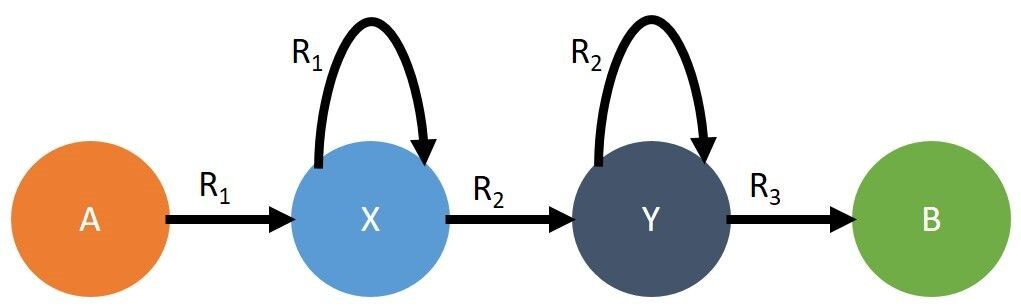
\includegraphics[width=100mm]{figs/chapter4/fig2.jpg}
    \end{center}
\label{ch4:fig:2}
\end{figure}

\begin{table}[htb]
    \caption[Lotka-Volterra System]{Lotka-Volterra System: The System Parameters
and Paths Used in the Iterative Solution Procedure.}
    \begin{center}
\begin{tabular}{clcc}
\rowcolor[HTML]{C0C0C0} 
\multicolumn{2}{c}{\cellcolor[HTML]{C0C0C0}reactions}               & rate coefficients    & initial conditions             \\
$R_1$                & $A+X \xrightarrow[]{} 2X$                    & $k_1 = 10$           & \multicolumn{1}{l}{$A(0)=1.0$} \\
$R_2$                & $X+Y \xrightarrow[]{} 2Y$                    & $k_2 = 10$           & \multicolumn{1}{l}{$B(0)=1.0$} \\
$R_3$                & $Y \xrightarrow[]{} B$                       & $k_3 = 10$           & \multicolumn{1}{l}{$X(0)=1.0$} \\
\multicolumn{1}{l}{} &                                              & \multicolumn{1}{l}{} & \multicolumn{1}{l}{$Y(0)=1.0$} \\
\rowcolor[HTML]{C0C0C0} 
path                 & \multicolumn{1}{c}{\cellcolor[HTML]{C0C0C0}} &                      & length                         \\
\multicolumn{3}{c}{$A$}                                                                    & 0                              \\
\multicolumn{3}{c}{$B$}                                                                    & 0                              \\
\multicolumn{3}{c}{$X$}                                                                    & 0                              \\
\multicolumn{3}{c}{$Y$}                                                                    & 0                              \\
\multicolumn{3}{c}{$A \rightarrow X$}                                                      & 1                              \\
\multicolumn{3}{c}{$X \rightarrow Y$}                                                      & 1                              \\
\multicolumn{3}{c}{$Y \rightarrow B$}                                                      & 1                              \\
\multicolumn{3}{c}{$A \rightarrow X \rightarrow Y$}                                        & 2                              \\
\multicolumn{3}{c}{$X \rightarrow Y \rightarrow B$}                                        & 2                              \\
\multicolumn{3}{c}{$A \rightarrow X \rightarrow Y \rightarrow B$}                          & 3                             
\end{tabular}
   \\ \rule{0mm}{5mm}
   ${}^\dagger$Concentration of A can vary with time.		% footnote symbol
\end{center}
\label{ch4:table1}
\end{table}

where $A$, $B$, $X$, and $Y$ stand for the time-dependent
concentrations, and $k_1$, $k_2$, and $k_3$ are the rate coefficients in
reactions \ref{ch4:lv:rxn1}, \ref{ch4:lv:rxn2} and \ref{ch4:lv:rxn3}. When we hold fixed the value of $A$, the
intermediates $X$ and $Y$ can undergo a variety of interesting
nonlinear effects such as persistent chemical oscillation. For the
autonomous LV problem, where $A$ varies in time, the kinetics
approaches a simple stable equilibrium state. Since reactions
\ref{ch4:lv:rxn1}, \ref{ch4:lv:rxn2} and \ref{ch4:lv:rxn3} conserve the number of molecules, we can hypothesize
a fictitious atom at the core of each species that we choose to
follow. The directed chemical graph, shown in Fig. \ref{ch4:fig:2}, illustrates the simple connectivity of the chemical mechanism.
We list in Table 1 the parameters used in the calculation and
the possible reaction routes followed by a fictitious atom. In the
pathway representation, the kinetics is represented by 10
independent chemical paths: three terminating on B

